\chapter{Events model}
\label{sec:events_model}

In this chapter, we will describe the second component of the hierarchial topology representation, which is its topology model.

\section{Execution model}
\label{sec:execution_model}

To simulate the execution of a sequence of jobs on a machine topology, we need to define the execution model. This model consists of several components.

The first component is machines. Machines can be divided into one or more machine types. Machines are organized in a topology, and the processing at each part of the system follows the rules set down in chapter \hyperref[sec:topology_model]{3.1}.

The second component is jobs. Jobs can be divided into one or more job types. For each job type, we can define the processing time on each machine type. We can also define the forbidden combinations of job types and machine types, and such job types can not execute on such machine types. This can affect possible paths through the topology, most prominently in parallel groups.

For each job, we can define several characteristics. The first one is release date, which is the time at which the job arrives at the system. The second one is due date, which is the time at which the job is expected to finish its execution. The third and final one is weight, which is a priority factor of the job.

Each job has its paths DAG. When a job starts its execution in the system, it starts at the source of its DAG. Whenever it finishes execution on a machine or group, it is moved to the next node in the DAG. When it reaches the sink of the DAG, the processing for it finishes.

The execution model is based on events. When the system starts, some events are created. The simulator consumes events one by one. Consumption of an event may lead to the creation of new events. The execution stops when there are no more events to consume. All the event types are described in chapter \hyperref[sec:event_types]{3.2.2}.

\section{Event types}
\label{sec:event_types}

There are a total of 22 event types, and they are all listed in Table \ref{tab:event_types}. Each event type is assigned a priority index, and the lower index means higher priority. In this case, the \textit{System exit} event has the highest priority, and the \textit{Wake machine} event has the lowest.

\begin{table}[!htbp]
    \begin{center}
        \begin{tabular}{|l|l|} 
         \hline
         Event type & Priority \\ [0.5ex] 
         \hline\hline
         System exit & 1 \\ 
         \hline
         System exit forced & 2 \\
         \hline
         System entry & 3 \\
         \hline
         Machine exit & 4 \\
         \hline
         Machine exit batch & 5 \\
         \hline
         Machine exit forced & 6 \\
         \hline
         Machine exit forced batch & 7 \\
         \hline
         Machine buffer entry & 8 \\
         \hline
         Prerequisites wait start & 9 \\
         \hline
         Prerequisites wait end & 10 \\
         \hline
         Preempt & 11 \\
         \hline
         Preempt batch & 12 \\
         \hline
         Setup start & 13 \\
         \hline
         Setup end & 14 \\
         \hline
         Setup cancel & 15 \\
         \hline
         Breakdown start & 16 \\
         \hline
         Breakdown end & 17 \\
         \hline
         Machine entry & 18 \\
         \hline
         Machine entry batch & 19 \\
         \hline
         Machine buffer entry request asynchronous & 20 \\
         \hline
         Machine buffer entry request synchronous & 21 \\
         \hline
         Wake machine & 22 \\
         \hline
        \end{tabular}
        \end{center}
        \caption{Event types and their priorities}
    \label{tab:event_types}
    \end{table}

When the system starts its execution, a priority queue is initialized with certain events. At each step of the execution, the first event is popped from the queue and consumed. Consummation of an events entails changing the internal state of the simulator, and possibly the creation of new events. This loop continues until there are no more events to consume, at which point the execution is finished. 

Each event has a timestamp, and they are ordered by it from lower to higher in the event queue. Ordering events by their respective timestamps ensures temporal consisency of the simulation.

Things get interesting when two events have an identical timestamp. Logically, this means that these events are happening at the same time. This is seemingly contradictory with the execution model which consumes events one by one. To resolve this, we apply several additional rules to the ordering of events in the event queue, to ensure a logical consistency of the simulation.

The first tie breaker is the topological order of components in the topology. They are ordered in a way that every component comes after all its predecessors, where predecessors of a component are a its parent in the topology tree, and the parent's predecessors. If two events share the same timestamp, they are then sorted using the topological order relations of their respective components. This ordering ensures that changes in the topology naturally propagate from its start to its end, and that, if a job is logically performing actions across multiple components at the same timestmap, it can fairly catch up to the last component where it needs to be, before scheduling decisions are made for that component. One situation where this behavior is prominent is if, after finishing processing at a machine, the job needs to go through several groups before it arrives to the next machine. Since processing in groups is instant and serves the purpose of directing the job towards its next component, a job can do a lot of actions at logically the same timestamp, and using the topological order of components as a tie breaker allows this behavior to be executed correctly.

The second tie breaker is the priority of events. If two events share the same timestamp and machine, then they are ordered by their priorities. This property, combined with the careful ordering of event types, also serves to ensure the logical consistency of the simulation.

Finally, if two events share the same timestmap, machine, and type, then it's irrelevant in which order they are executed. All the non-trivial decision making is being made in the \textit{Wake machine} event which has some interesting properties discussed later in this section, and that is the final puzzle piece to ensuring logical consistency among events with identical timestamps.

There are two types of events - auxilliary and principal. Auxilliary events are \textit{Machine buffer entry request asynchronous}, \textit{Machine buffer entry request synchronous} and \textit{Wake machine}, while the principal events are all the remaining event types. Principal events are used for advancing the job through its paths DAG, and they are crucial for the execution of a job. On the other hand, auxilliary events are useful only for the simulator. The purpose they serve is sending signals to machines, and as such, are not important for the execution of jobs.

Next, we will describe all event types, and how they utilized to simulate a certain execution aspect of jobs.

\subsection{System entry}
The \textit{System entry} event is triggered at the start of the execution of a job, and it corresponds to the source node in its paths DAG. This is one of the event types that the event queue is initialized with prior to the start of the simulation.

\subsection{System exit}
The \textit{System exit} event is triggered at the end of the execution of a job, and it corresponds to the sink node in its paths DAG.

\subsection{System exit forced}
The \textit{System exit forced} event is triggered when the execution of a job has to be forcefully terminated. The job does not reach the sink of its DAG, but still it is removed from the system.

\subsection{Machine buffer entry}
The \textit{Machine buffer entry} event happens when a job enters the buffer of a machine or a group. In terms of processing, groups are not differentiated from machines, so a job is processed on them as well, but this processing is instant and serves the function of directing the job to the next node in its paths DAG.

\subsection{Machine entry}
The \textit{Machine entry} event signifies the start of processing of a job on a machine. Whenever the machine is free and available for processing, it takes a job from its buffer and starts its processing.

\subsection{Machine exit}
The \textit{Machine exit} event signifies the end of processing of a job on a machine. At that point, the job is directed to the next node on its paths DAG by triggering a \textit{Machine buffer entry} or a \textit{System exit} event, and another job is taken for processing from the machine's buffer, if it is not empty.

\subsection{Machine exit forced}
The \textit{Machine exit forced} event is triggered when the execution of a job on a machine has to be forcefully terminated. After that, the \textit{System exit forced} event is triggered.

\subsection{Simulator feature: buffers}
Each machine has a buffer, and this buffer can have limited capacity. When a \textit{Machine exit} event is consumed, the next machine for that job is determined. If the next machine has space in its buffer, then the job is immediately moved to its buffer. Otherwise, the job is moved back to the buffer of its current machine to allow for processing of other jobs on this machine, where it stays until its next machine can accept it in its buffer. The minimal size of a buffer is one, because a job that is being processed still has a place reserved in the buffer in case it needs to be moved back to it. The \textit{Machine buffer entry} event reduces the buffer available capacity, and the \textit{Machine exit} event increases it. In between these two events, a job takes a place in the buffer, regardless of its stage of processing on the machine. 

\subsection{Machine buffer entry request asynchronous}
The auxilliary event \textit{Machine buffer entry request asynchronous} is used for this purpose. It sends a signal to a machine to check whether it can accept a job in its buffer. If the machine cannot accept the job at that moment, it remembers all unfulfilled entry requests, and acknowledges them when its buffer capacity frees up.

\subsection{Machine buffer entry request synchronous}
The auxilliary event \textit{Machine buffer entry request synchronous} is triggered by the \textit{System entry} event, and is used for entering the buffer of the root machine in the topology. If this machine cannot accept jobs in its buffer, then the job is declined, and the \textit{System exit forced} event is triggered instead, because there is no space prior to the root node buffer where the job could be kept until the buffer frees up. This request is synchronous because it required an immediate response, while the previous event was an asynchronous request, because it could be answered whenever the machine is ready to accept a job.

\subsection{Wake machine}
The auxilliary event \textit{Wake machine} is the central event type for this system. Events are severely limited in regards to the state of the simulator that they can change on their own. Most of the changes happen through this event, and this ensures logical consistency of the system. We can imagine a situation in which, at the same time, three jobs enter the system which contains a single machine, and are directed to its buffer. This means that between three \textit{Machine buffer entry} events and one \textit{Machine entry} event, something needs to happen, where the machine would choose which job it will process first. Since the events are consumed one by one, the first \textit{Machine buffer entry} event can not move the job from the machine buffer to processing, because it is not aware of other potential events which are logically happening at the same time, but due to the limitations of the computation model, will be consumed after this event. Instead what happens is that each \textit{Machine buffer entry} event triggers a \textit{Wake machine} event. This event is a signal to the machine, saying that an event has happened which may trigger a change in the machine's internal state. It has the lowest priority, because it needs to allow all other events to happen, before it has all the information it needs to make the correct decisions. In our example, this ensures that only after all the jobs enter the machine buffer at the same logical time but on different steps of the execution of the simulation, the scheduler will decide which job will be processed first, as now it has all the information it needs. The \textit{Wake machine} event is heavily utilized among all the remaining event types.

An interesting property that the \textit{Wake machine} event should posses is that its executions in an uninterrupted succession should be idempotent. By uninterrupted succession, we mean that at a given timestamp, these events are executed one by one, without any other event types in between. For such sequences, the first event is the one applying the changes to the machine's internal state, while the rest don't change its state, as there was no new information between this \textit{Wake machine} event and the last one.

\subsection{Simulator feature: prerequisites}
Each node in a job's paths DAG may have zero or more prerequisites defined. Each prerequisite is in the following format - job $x$ has to have been completed on the machine $y$ at least $z$ times, before this job can start processing on the machine. Since a job can visit a machine multiple times due to the rules set by route and open groups, it is possible to define a prerequisite that requires that a job be processed multiple times on a machine. When the job enters the machine's buffer, if its prerequisites are not all satisfied, it waits in a stand-by mode until all the prerequisites have become satisfied, at which point the job can be processed on the machine.

\subsection{Prerequisites wait start}
The \textit{Prerequisites wait start} event is triggered when a job enters a machine buffer and it has unfulfilled prerequisites on the corresponding node in its paths DAG.

\subsection{Prerequisites wait end}
Upon the consumption of the \textit{Machine exit} event, the simulator updates all unfulfilled prerequisites whose machine and job match the machine and job of the event. If the prerequisite becomes fulfilled, and if it was the last unfulfilled prerequisite blocking a job from executing on a machine, the \textit{Prerequisites wait end} event is triggered. Then, that job becomes ready for processing on that machine.

\subsection{Simulator feature: preemptions}
It is possible to define that a combination of machine type and job type support preemptions. In that case, the scheduler is allowed to interrupt the processing of a job, and start processing a different job. The processing time that the job had is not lost, and once the job starts processing again, it continues where it left off.

\subsection{Preempt}
The \textit{Preempt} event is triggered when a job is processing on a machine on which it can be preempted, and a job of a higher priority enters the machine buffer and becomes ready for processing. In that case, the job is preempted, and it can continue the processing later.

\subsection{Simulator feature: breakdowns}
For every machine, it is possible to define breakdowns, which are periods when the machine is not available for processing, for example due to a maintenance. Information about breakdowns is known in advance and available to schedulers for use when making decisions.

\subsection{Breakdown start}
The \textit{Breakdown start} event is triggered when a breakdown for a machine starts. Just like the \textit{System entry} events, the event queue is initialized with these events prior to the start of the simulation. If the machine is processing a job when the breakdown starts, then things get interesting. If the job can be preempted, the \textit{Preempt} event is triggered. Otherwise, the \textit{Machine exit forced} event is triggered. For this reason, a \textit{Machine exit} event has a higher priority than a \textit{Preempt} event. If the job finishes processing on a machine at the exact same time when the machine starts going into a breakdown, then we want to gracefully finish processing the job first. Considerations such as this one were used to define the priorities of event types, and their relations with one another.

\subsection{Breakdown end}
The \textit{Breakdown end} event is triggered when a breakdown for a machine ends. Then the machine can start processing jobs again, so if it has available jobs in its buffer, a \textit{Machine entry} event is triggered. This is the final event type with which the event queue is initialized prior to the start of the simulation.

\subsection{Simulator feature: setups}
A setup is a time period in which the machine is not processing any job, but is necessary for context switching from the previous job to the next one. The setup rules are defined for machine types, and they are presented in the following format - when switching from a job of type $x$ to a job of type $y$, the required setup takes $z$ time to complete. If $x$ is not specified, then the setup rule is active when starting the execution of any job of type $y$, regardless of the job type of the previous job which was processed on the machine. If $y$ is not specified, then the setup rule is active whenever the previous job was of type $x$, regardless of the type of the next job. If neither $x$ nor $y$ are specified, then the setup rule is active whenever a job starts processing on the machine. These rules are specified in an ordered list, and when a job starts executing, the simulator scans through the list, trying to find a match. The first setup rule that matches the situation becomes active, while the rest are discarded. If no matching setup rule is found, then a setup is not triggered.

\subsection{Setup start}
The \textit{Setup start} event is triggered when a setup starts. It is triggered before a \textit{Machine entry} event, but after making a decision which job will be processed next on the machine.

\subsection{Setup end}
The \textit{Setup end} event is triggered when a setup ends. It is triggered by the \textit{Setup start} event, and it triggers a \textit{Machine entry} event.

\subsection{Setup cancel}
The \textit{Setup cancel} event is triggered by a \textit{Breakdown start} event, if the breakdown occurs while a setup is active. Unlike with preemptions, the time that the machine spent on a setup is not recorded, and once the breakdown ends, the setup starts from the beginning. This was a deliberate design decision, and an argument could be made both for the setup cancel and setup preempt behaviors, but the setup cancel was chosen for this system.

\subsection{Simulator feature: batch processing}
For a machine type, it is possible to define batch processing behavior. Batch processing rules are presented in the following format - on a machine of type $x$, jobs of type $y$ can be processed in batch, and the maximum number of jobs in a batch is $z$. If batch processing is supported, when a job starts processing on a machine, the simulator goes to the buffer and tries to find jobs which could be processed in batch with the current job. If they are found, they are put on the machine along with the primary job for processing. The only requirement is that all the jobs which are processed at the same time have identical processing remaining times on the machine. Alternative behavior could be that the processing lasts as long as the longest remaining processing time of any job in the batch, but this could lead to undesirable effect such as the priority inversion. The situation is the same as the interaction between setups and breakdowns, an argument could be made for both behaviors, but one was chosen for this system. In all aspects, the secondary jobs in the batch mimic the primary job in the batch, because they are being processed at that time only because the primary job is being processed and the machine supports batch processing for their type.

\subsection{Machine entry batch}
The \textit{Machine entry batch} event is triggered by the \textit{Machine entry} event when the requirements for batch processing are satisfied. This event is triggered once for every secondary job in the batch, and this rule applies to all the remaining batch event types.

\subsection{Machine exit batch}
The \textit{Machine exit batch} event is triggered by the \textit{Machine exit} event when the primary job in the batch finished processing. Because jobs can be processed in a batch only if they have identical remaining processing times, when the primary job finished processing, all the other jobs in the batch should finish processing as well.

\subsection{Machine exit forced batch}
The \textit{Machine exit forced batch} event is triggered by the \textit{Machine exit forced} event when the primary job in the batch has to forcefully finish processing.

\subsection{Preempt batch}
The \textit{Preempt batch} event is triggered by the \textit{Preempt} event when the primary job in the batch is being preempted. Since preemption rules are defined for a machine type and job type combination, just as batch rules are, if the primary job in the batch can be preempted, the secondary ones can be as well.

\section{Interactions between events}

Figure \ref{fig:interactions_between_events} shows all event types, and their interactions. Black dots are sources, and the black dots with a red border are sinks. Full arrows imply that an event always triggers another event. Dashed arrows imply that an event may or may not trigger another event. White rhombuses imply branching, which means that an event always triggers one and exactly one of the events that the rhombus is connected to. This diagram was not created with any modelling standards such as the UML in mind, but instead, some ad hoc notations described earlier in this paragraph were used. 

Looking at the diagram, it is apparent that the \textit{Wake machine} event is at the centre of the whole system, and that the effects that the other event types can have without it are only local, like a \textit{Machine entry} event triggering a \textit{Machine exit} event. For example, even the \textit{Machine entry batch} events are not triggered directly by the \textit{Machine entry} event as was described in chapter \ref{sec:event_types}, but instead, this interaction happens through the \textit{Wake machine} event. Otherwise, the system could very easily become unmantainable, with unpredictable interactions. It is easier and more reliable to guarantee logical consistency if all the non-trivial decision making is concentrated in one place, rather than dispersed across the system.

[TODO: popraviti ovaj dijagram]
\begin{figure}[!htbp]
	\centering
	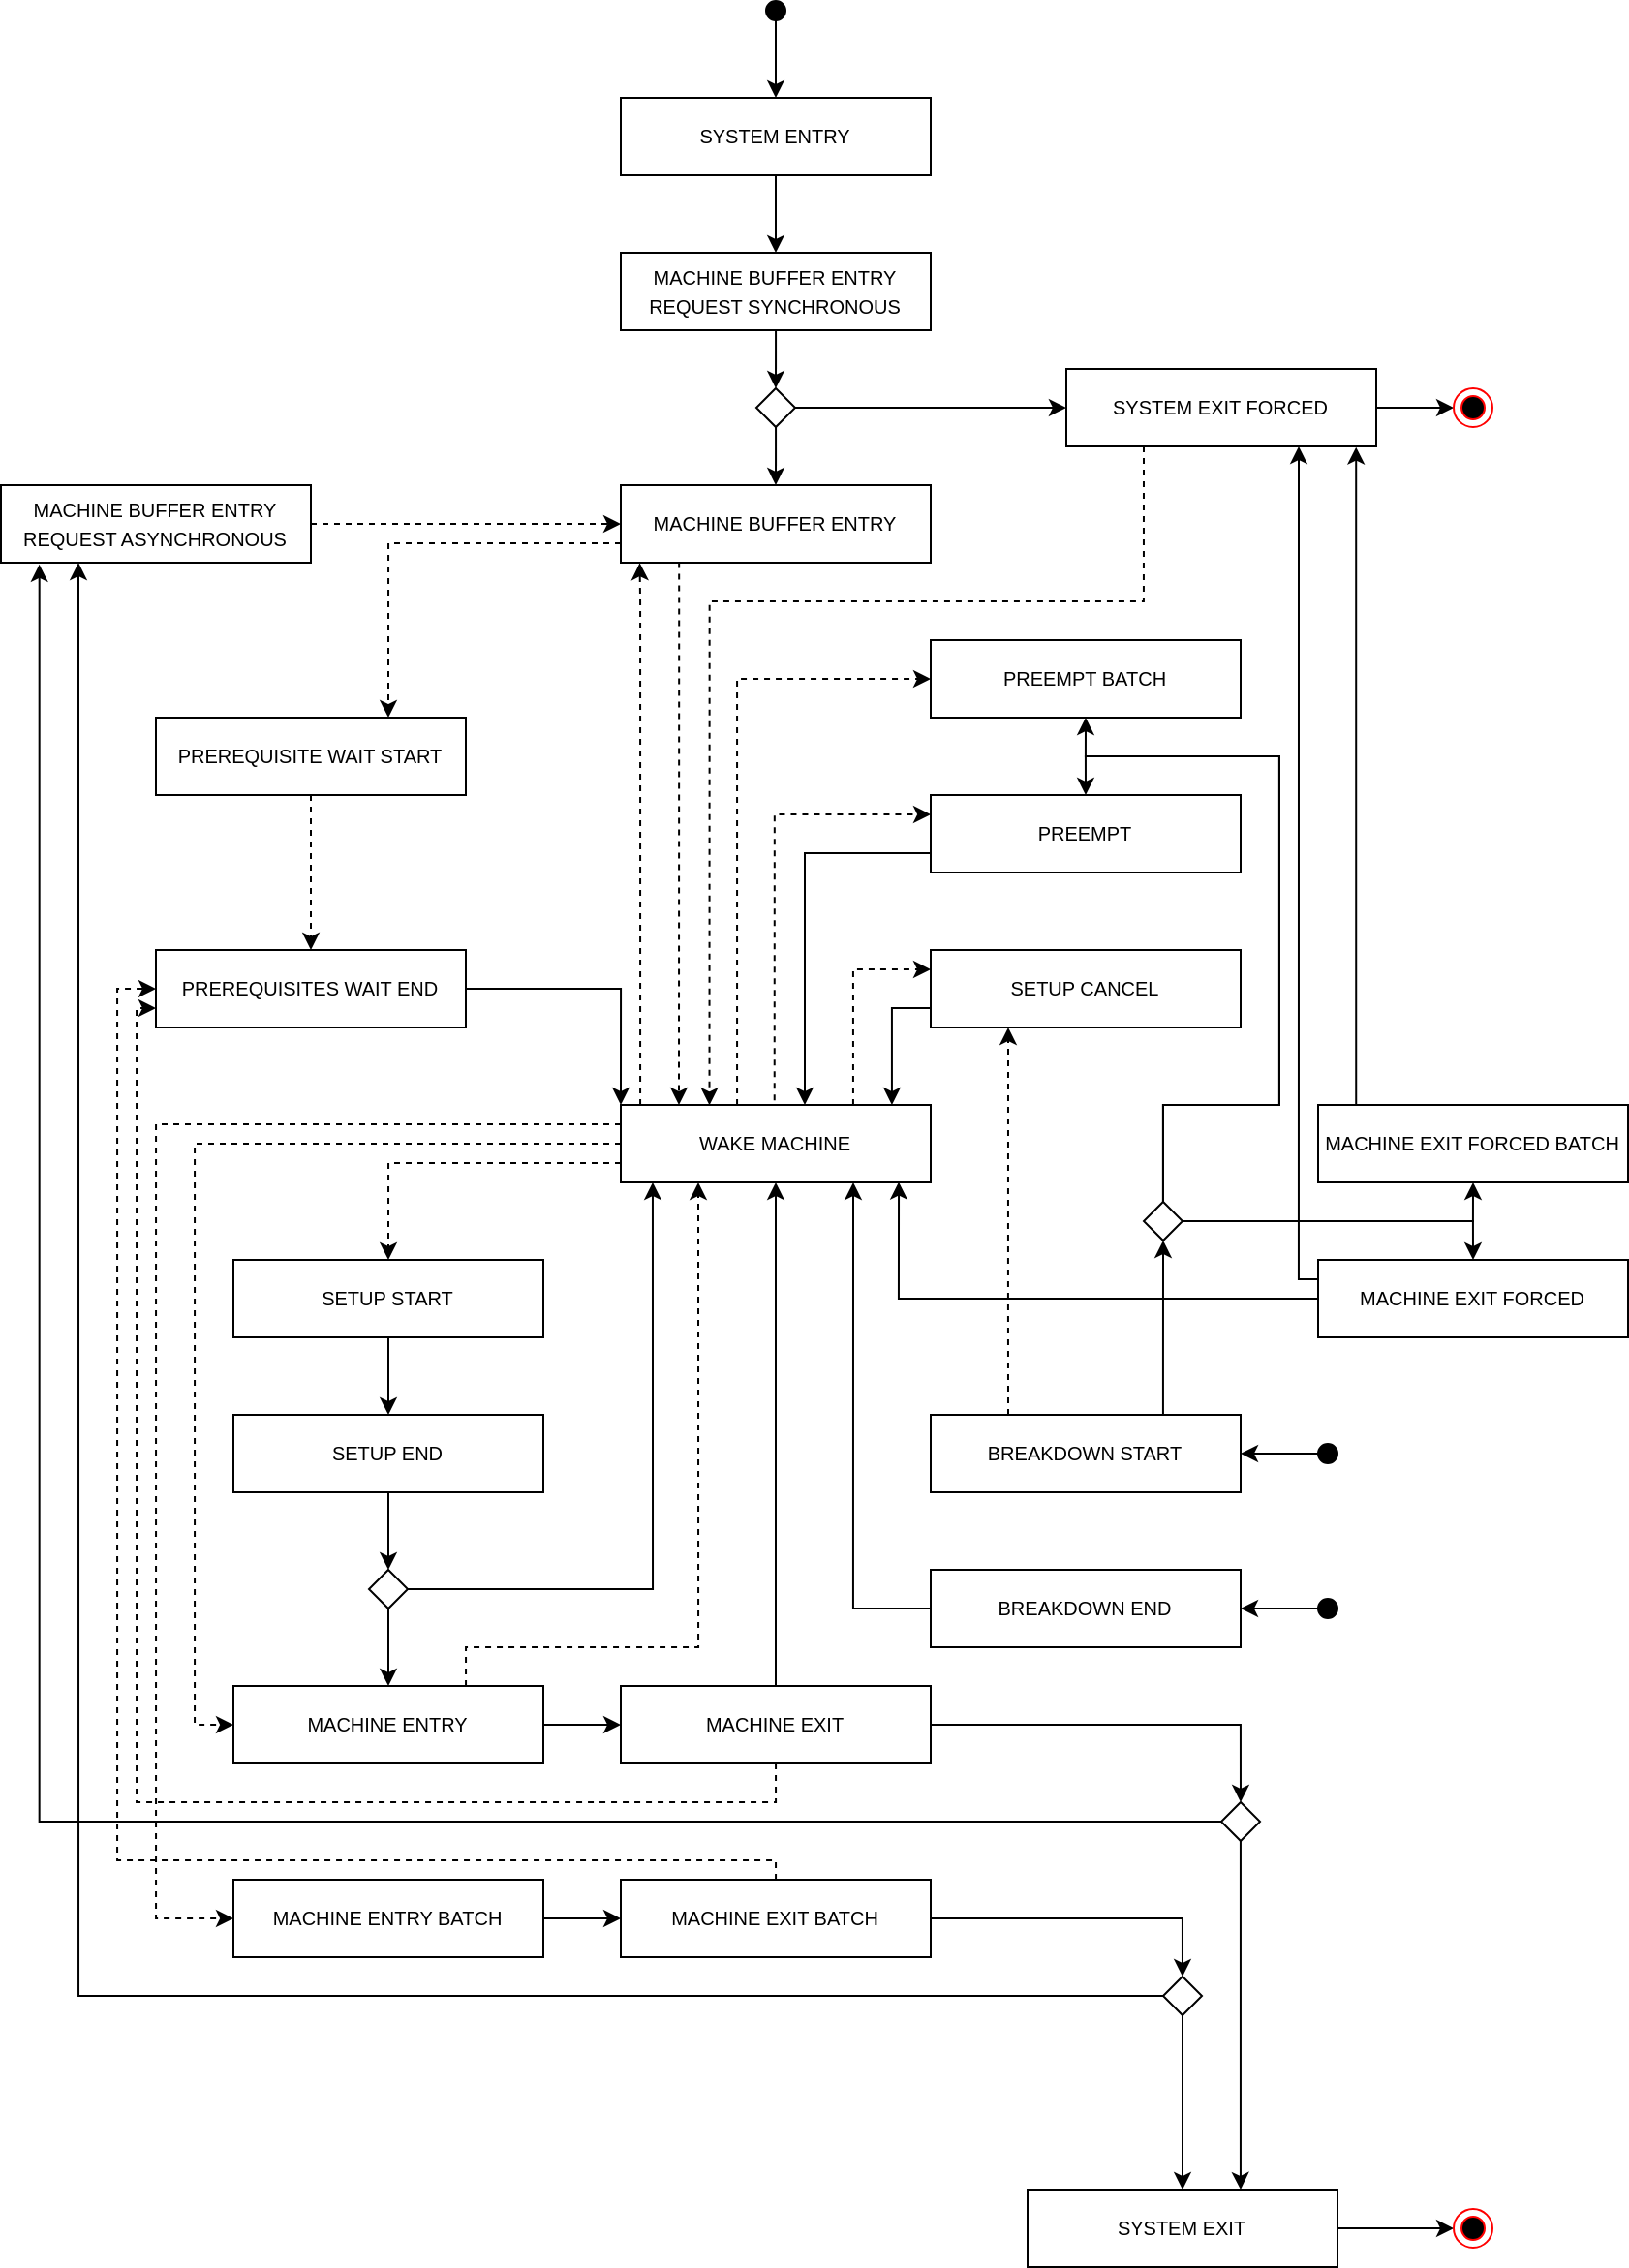
\includegraphics[scale=0.5]{../images/events.png}
	\caption{Interactions between events}
    \label{fig:interactions_between_events}
\end{figure}

\section{Execution examples}
\label{sec:execution_examples}

To demonstrate how events can be utilized to simulate the execution of a job in a topology, we will go through a couple of examples. In these examples, the auxilliary event types (\textit{Machine buffer entry request asynchronous}, \textit{Machine buffer entry request synchronous} and \textit{Wake machine}) will be excluded for simplicity, as they are not important for a job and its execution steps.

\subsection{Single machine}

Execution on the environment $1$ (single machine) can be simulated using the following sequence of events, where the machine has an identificator 1:
\begin{itemize}
    \item System entry
    \item Machine 1 buffer entry
    \item Machine 1 entry
    \item Machine 1 exit
    \item System exit
  \end{itemize}

\subsection{Flow shop}

Execution on the environment $F_3$ (flow shop with three machines, equivalent to a serial group) can be simulated using the following sequence of events, where a serial group has an identificator 1, and the machines have identificators 2-4:
\begin{itemize}
    \item System entry
    \item Machine 1 buffer entry
    \item Machine 1 entry
    \item Machine 1 exit
    \item Machine 2 buffer entry
    \item Machine 2 entry
    \item Machine 2 exit
    \item Machine 3 buffer entry
    \item Machine 3 entry
    \item Machine 3 exit
    \item Machine 4 buffer entry
    \item Machine 4 entry
    \item Machine 4 exit
    \item System exit
  \end{itemize}

\subsection{Parallel machines}

Execution on the environment $P_3$ (three machines in parallel) can be simulated using the following sequence of events, where a parallel group has an identificator 1, and the machines have identificators 2-4:
\begin{itemize}
    \item System entry
    \item Machine 1 buffer entry
    \item Machine 1 entry
    \item Machine 1 exit
    \item Machine 3 buffer entry
    \item Machine 3 entry
    \item Machine 3 exit
    \item System exit
  \end{itemize}

\section{Processing characteristics and constraints}
\label{sec:processing_characteristics_and_constraints}

The scheduling model described in \citep{pinedo2016scheduling} defines a number of processing characteristics and constraints. Here, we will go over each one of them, and describe how they can be achieved using our events model. In other words, here we will describe how our events model handles $\beta$ entries from the scheduling problem definition.

Release date ($r_j$) is the time at which the job $j$ enters the system and becomes ready for processing. This can be easily specified for every job, along with the due date ($d_j$) and weight ($w_j$) of the job.

Preemptions ($prmp$) are achieved using the \textit{Preempt} and \textit{Preempt batch} events.

Precedence constraints ($prec$) allow requiring that one or more jobs have to be completed before another job can start processing. They are achieved using the \textit{Prerequisites wait start} and \textit{Prerequisites wait end} events.

Sequence dependent setup times ($s_{jk}$) are what we have called setups earlier in this chapter, and they are achieved using the \textit{Setup start}, \textit{Setup end} and \textit{Setup cancel} events.

Job families ($fmls$) are equivalent to the job types mechanism. In this context, job families dictate the setup time between jobs, and this can be easily specified because our setup rules work with job types.

Batch processing ($batch(b)$) is achieved using the \textit{Machine entry batch}, \textit{Machine exit batch}, \textit{Machine exit forced batch} and \textit{Preempt batch} events.

Breakdowns ($brkdwn$) are achieved using the \textit{Breakdown start} and \textit{Breakdown end} events.

Machine eligibility restrictions ($M_j$) allow specifying which jobs cannot be processed on which machines. They are achieved by specifying the forbidden machine types for each job type.

Permutation ($prmu$) is a constraint in flow shop environments which requires that queues in front of each other operate according to the \textit{First In First Out (FIFO)} principle. This behavior is default in the serial group element.

Blocking ($block$) specifies that if a flow shop has buffers of a limited size between subsequent machines, when the upstream buffer is full, a machine is not allowed to release a job whose processing it has finished. This behavior is implemented in machine buffers with limited size.

No-wait ($nwt$) is a phenomenon which may occur in flow shops, where jobs are not allowed to wait between two successive machines. In other words, their processing in the flow shop needs to be uninterrupted between machines. This behavior can be achieved by specyfing that a serial group and all its components share the same buffer whose size is equal to one. In that case, only when a job leaves the serial group will the buffer free up and the serial group will be ready to accept another job.

Recirculation ($rcrc$) allows jobs to be processed on the same components multiple times. This behavior is allowed in route and open groups.

As we have demonstrated, the events model presented in this chapter is a versatile model which fully covers the processing characteristics and constraints of the machines and jobs scheduling model.